%
% fig-fluss.tex -- Darstellung des Flusses
%
% (c) 2024 Anna Pietak
%
\begin{figure}
    \centering
    \tikzset{every picture/.style={line width=0.75pt}} %set default line width to 0.75pt        

    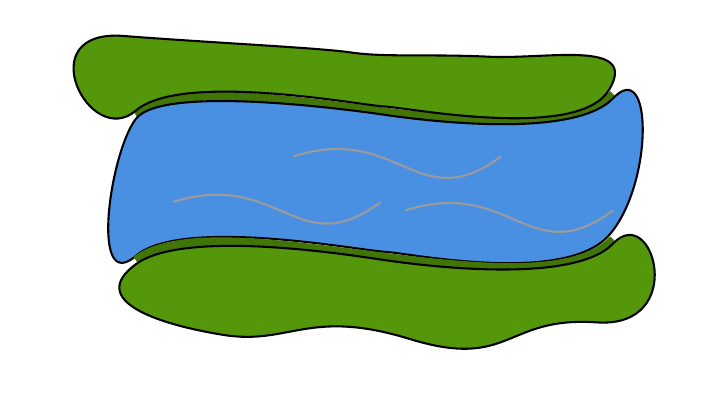
\begin{tikzpicture}[x=0.75pt,y=0.75pt,yscale=-1,xscale=1]
%uncomment if require: \path (0,300); %set diagram left start at 0, and has height of 300

%Curve Lines [id:da608977851192717] 
\draw [color={rgb, 255:red, 65; green, 117; blue, 5 }  ,draw opacity=1 ][line width=3]    (300,110) .. controls (340,80) and (493.51,138.06) .. (530,100) ;
%Shape: Polygon Curved [id:ds9392726871646548] 
\draw  [fill={rgb, 255:red, 74; green, 144; blue, 226 }  ,fill opacity=1 ] (300,112) .. controls (312.68,95.2) and (403.92,107.66) .. (420,110) .. controls (436.08,112.34) and (510.65,122.34) .. (530,102) .. controls (549.35,81.66) and (549.3,143.91) .. (528,168) .. controls (506.7,192.09) and (432.13,176.66) .. (420,176) .. controls (407.87,175.34) and (322.13,158.94) .. (300,178) .. controls (277.87,197.06) and (287.32,128.8) .. (300,112) -- cycle ;
%Curve Lines [id:da6433547723995421] 
\draw [color={rgb, 255:red, 65; green, 117; blue, 5 }  ,draw opacity=1 ][line width=3]    (300,180) .. controls (340,150) and (493.51,208.06) .. (530,170) ;
%Shape: Polygon Curved [id:ds34371397326569686] 
\draw  [fill={rgb, 255:red, 85; green, 151; blue, 11 }  ,fill opacity=1 ] (300,182) .. controls (323.56,164.66) and (403.92,177.66) .. (420,180) .. controls (436.08,182.34) and (510.65,192.34) .. (530,172) .. controls (549.35,151.66) and (566.44,213.06) .. (522,210) .. controls (477.56,206.94) and (481.01,233.06) .. (432,218) .. controls (382.99,202.94) and (374.13,221.23) .. (342,216) .. controls (309.87,210.77) and (276.44,199.34) .. (300,182) -- cycle ;
%Shape: Polygon Curved [id:ds3342416894164969] 
\draw  [fill={rgb, 255:red, 85; green, 151; blue, 11 }  ,fill opacity=1 ] (294,72) .. controls (339.58,75.49) and (387.92,77.66) .. (404,80) .. controls (420.08,82.34) and (442.15,80.63) .. (470,82) .. controls (497.85,83.37) and (542.72,73.49) .. (528,98) .. controls (513.28,122.51) and (432.13,106.66) .. (420,106) .. controls (407.87,105.34) and (322.13,88.94) .. (300,108) .. controls (277.87,127.06) and (248.42,68.51) .. (294,72) -- cycle ;
%Curve Lines [id:da7504908272245701] 
\draw [color={rgb, 255:red, 155; green, 155; blue, 155 }  ,draw opacity=1 ]   (318,152) .. controls (369.01,135.91) and (378,182) .. (418,152) ;
%Curve Lines [id:da01966435364089625] 
\draw [color={rgb, 255:red, 155; green, 155; blue, 155 }  ,draw opacity=1 ]   (376,130) .. controls (427.01,113.91) and (436,160) .. (476,130) ;
%Curve Lines [id:da5498107083025197] 
\draw [color={rgb, 255:red, 155; green, 155; blue, 155 }  ,draw opacity=1 ]   (430,156) .. controls (481.01,139.91) and (490,186) .. (530,156) ;




\end{tikzpicture}

    \caption{Fluss der überquert werden soll. Blau ist der Fluss eingezeichnet und grün das Ufer.}
    \label{fig:river_original}
\end{figure}
